% Journal of Cheminformatics (Springer Nature) format
\documentclass[twocolumn]{article}

\usepackage[utf8]{inputenc}
\usepackage[T1]{fontenc}
\usepackage{amsmath,amssymb}
\usepackage{graphicx}
\usepackage[colorlinks=true,citecolor=blue,linkcolor=blue,urlcolor=blue]{hyperref}
\usepackage{booktabs}
\usepackage{multirow}
\usepackage{xcolor}
\usepackage{siunitx}
\usepackage{natbib}
\usepackage{microtype}
\usepackage{geometry}
\geometry{margin=2cm}

% ============ Custom commands ============
\newcommand{\lam}{\lambda}
\newcommand{\lamhole}{\lambda_{\text{hole}}}
\newcommand{\lamcat}{\lambda_{\text{cation}}}
\newcommand{\lamtrip}{\lambda_{\text{triplet}}}
\newcommand{\thetaenc}{\theta_{\text{enc}}}
\newcommand{\thetahead}{\theta_{\text{head}}}
\newcommand{\Rsq}{R^{2}}
\newcommand{\FedPer}{\textsc{FedPer}}
\newcommand{\FedBN}{\textsc{FedBN}}
\newcommand{\FedAvg}{\textsc{FedAvg}}

\title{Personalized Federated Learning with Graph Neural Networks and Kolmogorov--Arnold Networks for Cross-Domain Molecular Reorganization Energy Prediction}

\author{
  Can Leng\textsuperscript{1} %
  \and Author Two\textsuperscript{1} %
}

\date{}

\begin{document}
\maketitle

% ================================================================
%  ABSTRACT
% ================================================================
\begin{abstract}
Molecular reorganization energy ($\lam$) is a critical descriptor governing charge-transfer rates in organic semiconductors, yet its accurate prediction remains challenging due to the fragmentation of relevant data across institutions with heterogeneous chemical domains and privacy constraints.
Small specialized laboratories, such as those studying thermally activated delayed fluorescence (TADF) emitters, often possess fewer than 50 molecules---a regime in which isolated local models fail catastrophically ($\Rsq < 0$).
Existing federated learning approaches for molecular property prediction have not addressed the compounded challenges of chemical domain shift, heterogeneous target quantities ($\lamcat$ vs.\ $\lamhole$ vs.\ $\lamtrip$), and the absence of three-dimensional conformational information.

This work presents \textbf{FedPer-KAN}, a personalized federated learning framework that combines a shared graph encoder---either the 2D Graph Isomorphism Network (GIN)~\cite{Xu2019_GIN} or the 3D continuous-filter SchNet~\cite{Schutt2018_SchNet}---with client-private Kolmogorov--Arnold Network (KAN)~\cite{KAN2024} regression heads under the \FedPer{}~\cite{Arivazhagan2019_FedPer}+\FedBN{}~\cite{Li2021_FedBN} aggregation strategy.
The framework is evaluated across four heterogeneous clients: Client~A (6{,}020 non-aromatic molecules, $\lamcat$), Client~B (9{,}190 aromatic molecules, $\lamcat$), Client~C (5{,}876 conjugated organic semiconductors, $\lamhole$), and Client~D (53 TADF molecules, $\lamhole / \lamtrip$).

Federated collaboration raises the large-client $\Rsq$ from 0.52 (local GIN+MLP) to 0.85 (federated GIN+KAN), with the KAN head outperforming MLP by 30.7\% in $\Rsq$.
For the data-scarce Client~D, $\Rsq$ improves from $-0.68$ (local) to $+0.03$ (federated 2D GIN) and $+0.18$ (federated 3D SchNet).
Systematic ablation studies and per-molecule error analysis reveal a fundamental information bottleneck in 2D graph representations for conformationally flexible TADF molecules: GIN prediction errors correlate with the number of rotatable bonds ($r = 0.30$, $p = 0.028$), whereas SchNet errors do not ($p = 0.256$), confirming that explicit 3D coordinate encoding is essential for capturing the torsional degrees of freedom that govern $\lam$.
These findings establish that personalized federated learning, when coupled with physically faithful 3D representations, provides a principled solution to both data fragmentation and domain heterogeneity in molecular property prediction.
\end{abstract}

\textbf{Keywords:} federated learning; reorganization energy; graph neural network; Kolmogorov--Arnold network; TADF; molecular property prediction

% ================================================================
%  SECTION 1: INTRODUCTION
% ================================================================
\section{Introduction}\label{sec:intro}

\subsection*{Reorganization energy: importance and prediction challenges}

Molecular reorganization energy ($\lam$) is the central parameter in Marcus theory of electron transfer~\cite{Marcus1993}, quantifying the energetic cost of nuclear rearrangement accompanying a charge-transfer event.
In organic semiconductors, $\lam$ directly governs the hopping rate $k_{\text{ET}} \propto \exp(-\lam / 4k_BT)$ and therefore controls carrier mobility in organic field-effect transistors~\cite{Coropceanu2007}, exciton dissociation efficiency in organic photovoltaics, and---critically for next-generation displays---the reverse intersystem crossing (rISC) rate in thermally activated delayed fluorescence (TADF) emitters~\cite{Uoyama2012_TADF}.
A low $\lam$ promotes rapid charge transport and efficient rISC, making $\lam$ a primary design target for high-performance organic electronic materials.

Computing $\lam$ from first principles requires two separate geometry optimizations at the density functional theory (DFT) level---one for the neutral state and one for the charged (cation, anion, or excited) state---followed by evaluation of single-point energies at the cross geometries~\cite{Nelsen1987}.
For molecules with more than 30 heavy atoms, this four-point procedure costs 10--100 CPU-hours per molecule, making large-scale screening prohibitively expensive.
Machine learning (ML) models offer a compelling alternative: graph neural networks (GNNs) trained on DFT-computed $\lam$ values can predict reorganization energies in milliseconds.
Recent work by Atahan-Evrenk and Atalay~\cite{AtahanEvrenk2019_RE} demonstrated random-forest regression on molecular fingerprints for 5{,}876 conjugated semiconductors, while Li and Tabor~\cite{Li2023_SchNet} achieved $\Rsq > 0.9$ using 3D SchNet~\cite{Schutt2018_SchNet} trained on approximately 50{,}000 molecules.
However, these successes rely on large, centralized datasets curated within a single laboratory---a luxury unavailable to most research groups.
While ML methods offer a promising path forward, their effectiveness depends critically on data availability---a condition that is rarely met in practice.

\subsection*{The data silo problem}

In practice, molecular $\lam$ data are fragmented across institutions.
Large-scale computational databases (e.g., QM9 derivatives) contain tens of thousands of small organic molecules, but the chemical space they cover rarely overlaps with the complex donor--acceptor architectures studied in specialized TADF laboratories.
These specialized labs often possess fewer than 100 molecules with DFT-quality $\lam$ values, a regime in which local model training fails catastrophically: our experiments show that training a GIN+KAN model on 53 TADF molecules yields $\Rsq = -0.68$ (Table~\ref{tab:summary}, E5).
Meanwhile, intellectual property concerns and privacy regulations prevent the direct pooling of proprietary molecular data across institutions.

Federated learning (FL)~\cite{McMahan2017_FedAvg} offers a principled solution to this dilemma: multiple clients collaboratively train a shared model by exchanging only model parameters---never raw data.
In the molecular sciences, FL would enable small TADF laboratories to exploit the representational knowledge encoded in large public databases without exposing their proprietary molecular structures.
Federated learning addresses the data sharing barrier, yet existing FL frameworks for molecular property prediction face two fundamental limitations.

\subsection*{Limitations of existing approaches}

Several recent studies have applied federated learning to molecular property prediction.
FedChem~\cite{FedChem2022} applied \FedAvg{}~\cite{McMahan2017_FedAvg} with message-passing neural networks but treated chemical domain shift as a secondary concern, assuming relatively homogeneous client distributions.
Heyndrickx et al.~\cite{Heyndrickx2023} reported federated multi-task learning using traditional molecular descriptors rather than learned graph representations.
FLAP~\cite{FLAP2023} explored federated pre-training for ADMET properties but did not address physically heterogeneous target quantities.
None of these works confronted the simultaneous challenges of (i) extreme chemical domain shift, (ii) heterogeneous physical target quantities ($\lamcat$ vs.\ $\lamhole$ vs.\ $\lamtrip$), and (iii) severe data imbalance (53 vs.\ 15{,}000 molecules).

A deeper limitation concerns the molecular representation itself.
Reorganization energy is fundamentally a geometric quantity: it measures the nuclear displacement between two equilibrium structures.
For TADF emitters, $\lam$ is dominated by large-amplitude donor--acceptor dihedral torsions (10--40$^{\circ}$ upon ionization), making it exquisitely sensitive to three-dimensional conformation.
Yet standard 2D GNNs such as the Graph Isomorphism Network (GIN)~\cite{Xu2019_GIN} operate exclusively on topological connectivity.
Their expressive power is bounded by the Weisfeiler--Leman (WL) graph isomorphism test~\cite{Xu2019_GIN}, which is provably blind to geometric features: two molecules with identical connectivity graphs but different spatial conformations---and hence vastly different $\lam$ values---are indistinguishable to the encoder.
This \emph{structural blindness} to out-of-plane torsion and steric repulsion constitutes a fundamental information bottleneck that no amount of federated data augmentation can overcome.
This observation motivates our systematic comparison of 2D GIN and 3D SchNet encoders within the federated framework.

In the extreme low-data regime characteristic of specialized laboratories---where $n < 100$ and conventional deep learning models overfit catastrophically---the choice of molecular representation becomes the decisive factor.
Neither data augmentation through federation nor architectural innovations in the regression head can compensate for the absence of geometric information when the property of interest is intrinsically three-dimensional.
This consideration elevates the encoder selection from a mere implementation detail to the central scientific question of the present study.

\subsection*{Contributions}

In summary, this paper makes the following contributions:
\begin{enumerate}
\item FedPer-KAN is proposed as the first personalized federated learning framework for cross-domain molecular reorganization energy prediction, combining shared GNN encoders with client-private KAN regression heads under \FedPer{}+\FedBN{} aggregation.
\item KAN regression heads are shown to outperform MLPs by 30.7\% in $\Rsq$ as local potential-energy-surface mappers, owing to their smooth B-spline approximation properties (Section~\ref{sec:kan_vs_mlp}).
\item A systematic diagnosis of the 2D representation bottleneck through four-hypothesis elimination establishes that conformational information---not data scarcity, target mismatch, or chemical-space divergence---is the primary limiting factor (Section~\ref{sec:bottleneck}).
\item Replacing GIN with 3D SchNet within the federated framework improves Client~D $\Rsq$ from $-0.031$ to $+0.181$, and subgroup analysis on rigid donor--acceptor molecules achieves $\Rsq = 0.852$ (Section~\ref{sec:subgroup}).
\item Personalized federation is found to outperform centralized training by physically isolating encoder representations from domain-specific regression mappings, preventing catastrophic interference between chemically incompatible clients (Section~\ref{sec:four_client}).
\end{enumerate}
The overall framework is illustrated in Fig.~\ref{fig:overview}.


% ================================================================
%  SECTION 2: RELATED WORK
% ================================================================
\section{Related Work}\label{sec:related}

\subsection{Machine Learning for Reorganization Energy}

Early ML approaches to $\lam$ prediction relied on hand-crafted molecular descriptors.
Atahan-Evrenk and Atalay~\cite{AtahanEvrenk2019_RE} trained gradient-boosted regression on extended connectivity fingerprints for 5{,}876 conjugated organic semiconductors, achieving mean absolute errors of approximately 0.03~eV for hole reorganization energy.
The advent of message-passing neural networks (MPNNs)~\cite{Gilmer2017_MPNN} enabled end-to-end learning on molecular graphs, eliminating the need for descriptor engineering.

Three-dimensional molecular representations offer a qualitatively richer input.
Sch\"utt et al.~\cite{Schutt2018_SchNet} introduced SchNet, which models interatomic interactions through continuous-filter convolutions on distance matrices, achieving the best-reported performance on QM9 molecular properties at the time.
Gasteiger et al.~\cite{Gasteiger2020_DimeNet} further incorporated angular information in DimeNet++, and Sch\"utt et al.~\cite{Schutt2021_PaiNN} proposed the equivariant PaiNN architecture.
Most relevant to our work, Li and Tabor~\cite{Li2023_SchNet} showed that SchNet trained on low-cost force-field conformers achieves $\Rsq > 0.9$ for $\lamcat$ prediction on a centralized dataset of ${\sim}50{,}000$ molecules.
Their success with approximate 3D geometries provides the key insight that motivates our adoption of SchNet in the federated setting.

We note that more expressive equivariant architectures---such as DimeNet++~\cite{Gasteiger2020_DimeNet}, which incorporates angular information through directional message passing, and PaiNN~\cite{Schutt2021_PaiNN}, which propagates equivariant feature vectors---have demonstrated improved accuracy on QM9 benchmarks.
In the present study, SchNet is deliberately chosen as the 3D encoder for two reasons.
First, our central scientific question concerns the information-theoretic gap between 2D topological and 3D spatial representations, rather than incremental accuracy gains among 3D architectures; SchNet provides a clean, well-characterized baseline for this comparison.
Second, SchNet's computational simplicity (scalar distance features only, no angular terms) is advantageous in the federated setting where communication efficiency and client-side computational constraints are practical considerations.
The substitution of SchNet with equivariant architectures represents a natural extension that we anticipate would further improve absolute accuracy, particularly for flexible molecules where angular features encode dihedral torsions more directly.

\subsection{Federated Learning for Molecular Properties}

Federated learning~\cite{McMahan2017_FedAvg} has been explored for drug discovery and molecular property prediction.
FedChem~\cite{FedChem2022} applied \FedAvg{} to molecular property prediction across pharmaceutical datasets, demonstrating improved generalization compared to local models.
FLAP~\cite{FLAP2023} introduced federated pre-training strategies for ADMET property prediction.
Heyndrickx et al.~\cite{Heyndrickx2023} presented a large-scale benchmark for federated multi-task learning on pharmaceutical data using traditional molecular descriptors.

Personalized federated learning addresses the non-IID data challenge inherent in heterogeneous chemical datasets.
\FedPer{}~\cite{Arivazhagan2019_FedPer} retains private prediction layers while sharing representation layers, which is architecturally natural for our encoder--head decomposition.
\FedBN{}~\cite{Li2021_FedBN} excludes batch normalization parameters from aggregation, addressing feature distribution shift across clients.
Our work is the first to combine these personalization strategies with GNN encoders for a physically motivated molecular property under extreme domain heterogeneity.

\subsection{Kolmogorov--Arnold Networks in Scientific Computing}

The Kolmogorov--Arnold representation theorem guarantees that any multivariate continuous function can be decomposed into compositions of univariate functions~\cite{KAN2024}.
KAN~\cite{KAN2024} operationalizes this theorem by placing learnable B-spline activation functions on network edges rather than fixed activations on nodes, enabling more expressive function approximation with fewer parameters.
KANs have shown promising results in scientific computing tasks including PDE solving and symbolic regression, where smooth, interpretable mappings are desirable.
Most recently, Li et al.~\cite{KAGNN2025} integrated KAN into GNN architectures at three levels (embedding, message passing, and readout), achieving improved performance on molecular benchmarks.
In the federated setting, Zhang et al.~\cite{FedLG2025} proposed a federated graph learning method for multi-party molecular discovery, though without KAN-based personalization.
To our knowledge, KAN has not been previously used as a client-private regression head in federated learning for molecular property prediction.
The smooth spline-based approximation of KAN is hypothesized to be particularly well-suited for this role, providing a compact yet expressive mapping from shared encoder representations to domain-specific target quantities.


% ================================================================
%  SECTION 3: METHODS
% ================================================================
\section{Methods}\label{sec:methods}

\subsection{Problem Formulation}\label{sec:formulation}

Consider $K$ clients, each holding a private dataset $\mathcal{D}_k = \{(\mathcal{G}_i^{(k)}, y_i^{(k)})\}_{i=1}^{n_k}$ of molecular graphs $\mathcal{G}$ and corresponding reorganization energies $y$.
The clients differ in chemical domain (covariate shift: non-aromatic, aromatic, conjugated semiconductors, TADF) and target physical quantity (concept shift: $\lamcat$, $\lamhole$, $\lamtrip$).
The global federated objective is:
\begin{equation}\label{eq:fed_obj}
  \min_{\thetaenc} \sum_{k=1}^{K} \frac{n_k}{N} \mathcal{L}_k(\thetaenc, \thetahead^{(k)}),
\end{equation}
where $N = \sum_k n_k$, $\thetaenc$ denotes shared encoder parameters, and $\thetahead^{(k)}$ denotes client-private regression head parameters.
The local loss $\mathcal{L}_k$ is the mean squared error over $\mathcal{D}_k$.

\subsection{Molecular Graph Construction}\label{sec:graph}

\paragraph{2D molecular graphs.}
Given a SMILES string, we construct a PyTorch Geometric~\cite{RDKit2023} graph $\mathcal{G} = (\mathbf{X}, \mathbf{E}, \mathbf{A})$.
Node features $\mathbf{x}_i \in \mathbb{R}^{11}$ comprise: atomic type one-hot encoding (C, N, O, S, F, Cl, Br, Other; 8 dimensions), normalized degree (1 dimension), formal charge (1 dimension), and Gasteiger partial charge (1 dimension).
Edge features $\mathbf{e}_{ij} \in \mathbb{R}^{4}$ encode bond type (single, double, triple, aromatic).
Six global molecular descriptors (molecular weight, TPSA, LogP, number of aromatic rings, maximum absolute partial charge, and molar refractivity) are concatenated to the graph-level representation after pooling.

\paragraph{3D molecular representation.}
For SchNet, we generate 3D conformers using the RDKit ETKDG algorithm~\cite{RDKit2023} followed by MMFF94 force-field optimization.
Each atom is represented by its nuclear charge $Z_i$ and Cartesian position $\mathbf{r}_i \in \mathbb{R}^3$.
This procedure requires only milliseconds per molecule and is compatible with the federated setting: each client independently computes atomic coordinates without sharing molecular structures.

\subsection{Model Architecture}\label{sec:architecture}

\paragraph{GIN encoder.}
The 2D encoder follows the Graph Isomorphism Network (GIN) architecture~\cite{Xu2019_GIN}, consisting of 5 GINConv layers with hidden dimension 300, each followed by batch normalization and ReLU activation.
Jumping Knowledge (JK) concatenation of all layer outputs is applied, followed by global mean + max pooling.
A linear projection maps the pooled representation to a 256-dimensional embedding $\mathbf{h} \in \mathbb{R}^{256}$.

\paragraph{SchNet encoder.}
The 3D encoder uses SchNet~\cite{Schutt2018_SchNet} with 6 interaction blocks, 256 atom-wise features, 128 filters, and a Gaussian radial basis expansion with 50 functions and a cutoff of 7.5~\AA{}.
Atom features are initialized from learnable embeddings of the nuclear charge $Z$.
Continuous-filter convolutions model pairwise interactions as:
\begin{equation}
  \mathbf{x}_i^{(l+1)} = \mathbf{x}_i^{(l)} + \sum_{j \in \mathcal{N}(i)} \mathbf{W}^{(l)} \mathbf{x}_j^{(l)} \circ \text{cfconv}(\|\mathbf{r}_i - \mathbf{r}_j\|),
\end{equation}
where cfconv denotes the continuous filter parametrized by the interatomic distance.
Global mean pooling produces a 256-dimensional graph representation.

\paragraph{KAN regression head.}\label{sec:kan_head}
The client-private regression head is a Kolmogorov--Arnold Network (KAN)~\cite{KAN2024} consisting of three KANLinear layers: $256 \to 64 \to 32 \to 1$, each using B-spline basis functions of order 3 with grid size 5 (optimized via ablation; Section~\ref{sec:ablation}).
Unlike conventional MLPs that apply fixed activation functions at nodes, KAN places learnable univariate functions $\phi_{q,p}$ on every edge:
\begin{equation}
  \text{KAN}(\mathbf{x}) = \sum_{q=1}^{n_2} \phi_{q,\cdot}\!\left(\sum_{p=1}^{n_1} \phi_{\cdot,p}(x_p)\right),
\end{equation}
where each $\phi$ is parametrized as a B-spline.

The physical motivation for choosing KAN over MLP as the client-private head is twofold.
First, B-spline basis functions provide \emph{locally smooth} approximations that act as implicit regularizers, preventing the catastrophic overfitting that afflicts MLPs on small datasets (53 molecules in Client~D).
Second, the functional decomposition aligns with the physics of $\lam$ prediction: the shared encoder learns \emph{universal spatial intuition}---transferable representations of interatomic distances and molecular topology---while each KAN head learns a \emph{domain-specific potential-energy-surface (PES) mapping} from these representations to the particular reorganization process ($\lamcat$, $\lamhole$, or $\lamtrip$) relevant to its client.
This encoder--head decomposition mirrors the separation between general chemical features (shared) and domain-specific energy landscapes (private), preventing the small-sample client from being overwhelmed by the large-sample client's optimization landscape.

\paragraph{MLP regression head (baseline).}
For comparison, the MLP head consists of Linear($256 \to 128$) $\to$ ReLU $\to$ Dropout(0.3) $\to$ Linear($128 \to 64$) $\to$ ReLU $\to$ Dropout(0.3) $\to$ Linear($64 \to 1$).

\subsection{Federated Strategy: \FedPer{} + \FedBN{}}\label{sec:fedstrategy}

Our aggregation protocol combines two personalization mechanisms.

\paragraph{\FedPer{}.}
Following Arivazhagan et al.~\cite{Arivazhagan2019_FedPer}, we partition the model into shared layers (encoder $\thetaenc$) and personalized layers (regression head $\thetahead^{(k)}$).
At each communication round $t$, only the encoder parameters are aggregated:
\begin{equation}
  \thetaenc^{(t+1)} = \sum_{k=1}^{K} \frac{n_k}{N} \thetaenc^{(k,t)},
\end{equation}
while each client's KAN head $\thetahead^{(k)}$ remains local.
This ensures that the domain-specific PES mapping is never contaminated by data from chemically incompatible clients.

\paragraph{\FedBN{}.}
Following Li et al.~\cite{Li2021_FedBN}, we additionally exclude all batch normalization parameters ($\gamma$, $\beta$, running mean, running variance) from aggregation.
Batch normalization statistics reflect the local feature distribution; aggregating them across clients with vastly different molecular compositions (e.g., small non-aromatic molecules vs.\ large TADF donor--acceptor systems) would destroy the normalization benefit.
The complete communication protocol is depicted in Fig.~\ref{fig:workflow}.

\subsection{Per-Client Label Normalization}\label{sec:labelnorm}

The four clients exhibit dramatically different label distributions: Client~A $\lamcat \in [0.01, 2.94]$~eV ($\mu = 0.72$~eV), Client~C $\lamhole \in [0.08, 0.87]$~eV ($\mu = 0.17$~eV), and Client~D $\lamhole \in [0.45, 3.00]$~eV ($\mu = 1.18$~eV).
To prevent the loss landscape from being dominated by clients with large absolute label values, we apply per-client z-score normalization: $\tilde{y}_i^{(k)} = (y_i^{(k)} - \mu_k) / \sigma_k$.
Predictions are denormalized before evaluation.
This normalization is physically motivated: the ``difficulty'' of predicting a reorganization energy should depend on the relative accuracy within each client's chemical domain, not on the absolute magnitude of $\lam$.


% ================================================================
%  SECTION 4: EXPERIMENTAL SETUP
% ================================================================
\section{Experimental Setup}\label{sec:setup}

\subsection{Datasets}\label{sec:datasets}

Four clients representing distinct chemical domains and physical target quantities are constructed (Fig.~\ref{fig:dataset}, Fig.~\ref{fig:tsne}):

\textbf{Client~A} (6{,}020 molecules): non-aromatic organic molecules derived from the QM9 dataset, with cation reorganization energy ($\lamcat$) computed at the B3LYP/6-31G(d) level.
These molecules contain 2--9 heavy atoms, predominantly aliphatic chains and small rings.

\textbf{Client~B} (9{,}190 molecules): aromatic organic molecules from the same QM9-derived database.
The aromatic ring criterion (NumAromaticRings $\geq 1$) produces molecules with $\pi$-conjugated systems, benzene derivatives, and heterocycles.

\textbf{Client~C} (5{,}876 molecules): conjugated organic semiconductors from the dataset of Atahan-Evrenk and Atalay~\cite{AtahanEvrenk2019_RE}, with hole reorganization energy ($\lamhole$) computed at the B3LYP/6-31G(d,p) level.
These molecules are larger (10--40 heavy atoms) and include many structures relevant to organic electronics.

\textbf{Client~D} (53 molecules): TADF emitters synthesized and characterized in our laboratory, with $\lamhole$ and $\lamtrip$ computed at the $\omega$B97XD/def2-TZVP level using the four-point adiabatic potential energy surface method.
These donor--acceptor molecules feature twisted $\pi$-systems with 8--24 heavy atoms.

\paragraph{Non-IID characterization.}
The four-client federation exhibits a dual extreme shift.
The \emph{covariate shift} spans from simple aliphatic molecules (Client~A) to complex TADF donor--acceptor architectures (Client~D), as visualized by the clearly separated clusters in the t-SNE embedding of Morgan fingerprints (Fig.~\ref{fig:tsne}).
The \emph{concept shift} is equally severe: $\lamcat$ describes nuclear relaxation from neutral to cation geometry (bond-length alternation dominates for rigid molecules); $\lamhole$ involves hole injection into the HOMO orbital (often dominated by dihedral torsion in conjugated systems); and $\lamtrip$ involves spin-forbidden excitation followed by excited-state relaxation (a qualitatively different potential energy surface).
These three physical processes probe different regions of the Born--Oppenheimer surface, making the mapping from molecular structure to $\lam$ client-specific even for structurally similar molecules.

A natural question is whether additional molecular property datasets---for instance, ADMET benchmarks from drug discovery---could further validate the framework.
However, reorganization energy is a fundamentally distinct physical quantity that requires computationally prohibitive four-point DFT geometry optimizations (two equilibrium structures and two single-point energies per molecule).
Standard drug discovery benchmarks such as MoleculeNet lack these high-fidelity $\lam$ labels entirely.
The four-client configuration used here---spanning aliphatic, aromatic, conjugated semiconductor, and TADF chemical domains---represents the current frontier of available DFT-quality reorganization energy data in the organic electronics literature.
Extension to additional $\lam$ datasets would require new DFT campaigns, which we identify as an important direction for future work.

\subsection{Implementation Details}\label{sec:implementation}

All experiments use PyTorch 2.4 and PyTorch Geometric on two NVIDIA A30 GPUs (24~GB each).
Client~A trains on GPU~0; Clients~B, C, and D train on GPU~1; federated aggregation runs on CPU.
The optimizer is Adam with learning rate $10^{-3}$ for SSL pre-training and $10^{-4}$ for supervised fine-tuning, combined with cosine annealing.
Batch sizes are 512 for Clients~A, B, and C, and full-batch for Client~D.
Early stopping with patience 15 on validation loss prevents overfitting.
Federated communication runs for 30 rounds with 5 local epochs per round.

\subsection{Evaluation Protocol}\label{sec:evaluation}

For Clients~A, B, and C, we report mean $\pm$ standard deviation over 5-fold random cross-validation.
For Client~D, we use leave-one-out cross-validation (LOOCV) due to the small sample size ($n = 53$ for $\lamhole$, $n = 49$ for $\lamtrip$), reporting $\Rsq$, MAE, and RMSE on the aggregated predictions.
LOOCV represents the most stringent evaluation protocol: each molecule is predicted by a model trained without it, avoiding any data leakage.

\subsection{Experiment Matrix}\label{sec:exp_matrix}

The 15 experiments (Table~\ref{tab:summary}) are organized into five groups: (i) local baselines with MLP and KAN heads (E1--E5), (ii) federated strategies---\FedAvg{}, \FedPer{}, \FedPer{}+\FedBN{}---with GIN+KAN (E6--E8), (iii) self-supervised pre-training with AtomMask, EdgePred, and GraphCL (E9--E11), (iv) four-client expansion and centralized upper bound (E12--E13), and (v) 3D SchNet variants (E14--E15).
Four ablation studies examine KAN grid size, SSL rounds, data fraction, and communication rounds.


% ================================================================
%  SECTION 5: RESULTS AND DISCUSSION
% ================================================================
\section{Results and Discussion}\label{sec:results}

\subsection{KAN vs.\ MLP Regression Heads}\label{sec:kan_vs_mlp}

The KAN and MLP regression heads are first compared under identical local training conditions (no federation).
On Client~A, replacing the MLP head (E1: $\Rsq = 0.523 \pm 0.059$) with a KAN head (E4: $\Rsq = 0.683 \pm 0.026$) yields a relative improvement of 30.7\% in $\Rsq$ (Fig.~\ref{fig:kan_vs_mlp}).
The improvement is consistent across clients: Client~B increases from $\Rsq = 0.686$ (E2, MLP) to $\Rsq = 0.726$ (implied by federated gains), and Client~D $\lamhole$ shifts from $\Rsq = -0.640$ (E3, MLP) to $\Rsq = -0.677$ (E5, KAN)---still negative, but with lower MAE (0.410 vs.\ 0.435~eV).

The KAN advantage is most pronounced on the data-rich clients where sufficient training data allows the spline basis functions to be accurately fitted.
On Client~D, both heads perform poorly in isolation ($\Rsq < 0$), confirming that 53 molecules are insufficient for local GNN training regardless of the head architecture.
The KAN's advantage manifests primarily in the federated setting, where the shared encoder provides a sufficiently rich 256-dimensional representation and the KAN head needs only to learn the local PES mapping---a lower-dimensional and smoother function that B-spline bases can approximate effectively even with limited local data.

\subsection{Federated Strategy Comparison}\label{sec:fed_strategy}

Four training paradigms for GIN+KAN are compared: local training (E4/E5), \FedAvg{} (E6), \FedPer{} (E7), and \FedPer{}+\FedBN{} (E8).

\FedAvg{} (E6: $\Rsq_\text{A} = 0.660$, $\Rsq_\text{B} = 0.789$) already improves over local baselines by enabling cross-client representation learning.
However, \FedAvg{} forces all clients to share a single regression head, causing gradient conflicts between the chemically disparate loss landscapes.
Client~D suffers most: $\Rsq_{\text{D,h}} = -0.507$, only marginally better than the local baseline.

\FedPer{} (E7) dramatically improves results by keeping the KAN heads private: $\Rsq_\text{A} = 0.777$, $\Rsq_\text{B} = 0.865$, $\Rsq_{\text{D,h}} = -0.108$.
The encoder benefits from the combined training signal of all clients, while each client's head specializes to its local energy landscape.

Adding \FedBN{} (E8) provides a further boost for Client~D: $\Rsq_{\text{D,h}} = +0.028$, crossing from negative to positive $\Rsq$ for the first time.
The client-private batch normalization statistics adapt to the drastically different molecular feature distributions (e.g., mean atomic mass, degree distributions) that characterize each client's chemical domain.
For the large clients, \FedBN{} shows marginal differences ($\Rsq_\text{A} = 0.750$, $\Rsq_\text{B} = 0.854$), indicating that the benefit is concentrated on the out-of-distribution client.

Having established \FedPer{}+\FedBN{} as the optimal federation strategy, the next question is whether self-supervised pre-training can further improve the shared encoder representations.

\subsection{Self-Supervised Pre-training}\label{sec:ssl}

Three self-supervised learning (SSL) pre-training strategies are evaluated for the GIN encoder before federated fine-tuning: AtomMask (E9), EdgePred (E10), and GraphCL~\cite{You2020_GraphCL} (E11).

AtomMask randomly masks 15\% of node features and trains the encoder to reconstruct atom types (cross-entropy) and Gasteiger charges (MSE).
EdgePred deletes 20\% of edges and trains a binary classifier on positive (deleted) and negative (non-existent) edges.
GraphCL generates two augmented views via node feature masking and edge deletion, then optimizes an InfoNCE contrastive loss~\cite{Hu2020_SSL}.

All three SSL methods improve the encoder's representational quality on large clients ($\Rsq_\text{A} \approx 0.73$, $\Rsq_\text{B} \approx 0.84$) relative to random initialization (Fig.~\ref{fig:strategies}b).
However, the gains on Client~D are inconsistent: AtomMask yields $\Rsq_{\text{D,h}} = -0.085$, EdgePred yields $-0.057$, and GraphCL yields $-0.258$.
The negative $\Rsq$ values indicate that SSL pre-training, while beneficial for learning general molecular representations, does not resolve the fundamental information bottleneck for TADF molecules.
This outcome can be attributed to the nature of the SSL tasks: AtomMask and EdgePred capture local chemical motifs (atom types, bond connectivity) that are well-represented in the 2D graph, while the critical information for $\lam$---torsional flexibility and 3D conformation---remains absent from the input.

\subsection{Four-Client Federation and Centralized Upper Bound}\label{sec:four_client}

\paragraph{Four-client expansion.}
To test whether including a physically matched client would benefit Client~D, we expanded the federation from three clients (A, B, D) to four (A, B, C, D) by adding Client~C---5{,}876 conjugated semiconductors predicting $\lamhole$, the same physical quantity as Client~D.
Experiment E12 (\FedPer{}+\FedBN{}, 4-client, GIN+KAN) yields $\Rsq_{\text{C}} = 0.833$, $\Rsq_{\text{D,h}} = -0.031$.
Client~C achieves strong performance, but Client~D does not improve compared to E8 ($\Rsq_{\text{D,h}} = +0.028$).
This confirms that the bottleneck is representational, not data-related: even 5{,}876 additional $\lamhole$ examples from a related chemical domain cannot compensate for the missing 3D conformational information.

\paragraph{Centralized upper bound.}
A natural question is whether centralized training---pooling all data and training a single model---would outperform the federated approach.
A centralized SchNet+KAN model was trained on the combined datasets of all four clients, with evaluation on Client~D via LOOCV.
Contrary to expectation, the centralized model achieves $\Rsq_{\text{D,h}} = -0.004$ (Table~\ref{tab:summary}), \emph{worse} than the federated SchNet result ($\Rsq = +0.181$, E14).

The physical explanation is illuminating.
Centralized training forces a single global model to simultaneously fit two fundamentally incompatible relaxation modes: Client~C molecules (conjugated semiconductors) undergo $\lamhole$ changes driven primarily by bond-length alternation---small, symmetric distortions of the $\pi$-backbone with $\lam \in [0.08, 0.87]$~eV.
Client~D molecules (TADF emitters), by contrast, undergo $\lamhole$ changes dominated by massive donor--acceptor dihedral torsions---large-amplitude, asymmetric distortions with $\lam \in [0.45, 3.00]$~eV.
A globally shared regression head lacks the expressive capacity to simultaneously map these two qualitatively different potential energy surface topologies: the bond-alternation regime of conjugated semiconductors occupies a fundamentally different region of the structure--energy manifold than the dihedral-torsion regime of TADF emitters.
Moreover, the gradient contributions from the 5{,}876 Client~C molecules dominate those from the 53 Client~D molecules by two orders of magnitude, systematically biasing the global model toward the bond-alternation regime and effectively silencing the minority client.

\FedPer{} resolves this catastrophic interference through architectural isolation: the shared encoder distills general distance--energy relationships common to all relaxation modes, while each client's private KAN head independently specializes to its local PES topology without cross-client gradient contamination.
This result furnishes a compelling \emph{a posteriori} justification for personalized federation: it is not merely a privacy-preserving surrogate for centralized training, but a fundamentally superior architecture for physically heterogeneous multi-domain learning where domain-specific nonlinearities must be preserved.

To summarize: the centralized SchNet model achieves $\Rsq_{\text{D,hole}} = -0.004$, whereas the federated SchNet (E14) achieves $\Rsq = +0.181$---a reversal of the conventional expectation that centralized training with more data should outperform distributed approaches.
This counter-intuitive result arises because personalized federation provides architectural isolation of incompatible potential energy surfaces, a benefit that no amount of additional pooled data can replicate when the underlying physics of relaxation differs qualitatively across clients.

\subsection{Ablation Studies}\label{sec:ablation}

Four ablation studies were conducted to characterize the sensitivity of the framework to key hyperparameters, focusing on Client~D $\lamhole$ performance (Fig.~\ref{fig:ablation}).

\paragraph{(a) KAN grid size.}
Varying the B-spline grid from 3 to 10 (at fixed spline order 3), we find that performance generally improves with grid resolution: grid 3 yields $\Rsq = -0.07$, grid 5 yields $-0.14$, grid 8 yields $-0.04$, and grid 10 yields $-0.02$.
The non-monotonic behavior at grid 5 likely reflects sensitivity to the spline basis in the small-sample regime, but the overall trend favors finer grids; gains plateau beyond grid 10 as the limited Client~D data cannot support higher-resolution splines without overfitting.

\paragraph{(b) SSL pre-training rounds.}
Sweeping the number of federated SSL pre-training rounds from 0 to 40, we observe an initial improvement from 0 rounds ($\Rsq = -0.10$) to 10 rounds ($\Rsq = -0.01$), followed by a slight decline at 20 rounds ($\Rsq = -0.06$) and recovery at 40 rounds ($\Rsq = +0.02$).
The modest and non-monotonic effect confirms that SSL primarily benefits the encoder's general molecular representations, while the Client~D bottleneck lies in the 2D$\to$3D information gap.

\paragraph{(c) Client~D data fraction.}
Reducing the local Client~D dataset from 100\% to 20\% (10 molecules), $\Rsq$ degrades from $-0.018$ to $-1.90$ under the same federated GIN+KAN configuration.
This steep decline shows that while federation provides substantial knowledge transfer from large clients, the local fine-tuning still requires a minimum critical mass of domain-specific examples to calibrate the private KAN head.

\paragraph{(d) Communication rounds.}
Increasing communication rounds from 5 to 30, Client~D $\Rsq$ improves from $-0.14$ to $+0.01$, with the majority of the gain occurring in the first 20 rounds.
This suggests that the encoder converges relatively quickly on the large-client representations, while the private KAN heads require continued local fine-tuning.
Accordingly, 30 rounds are used in all subsequent experiments.

% ================================================================
%  SECTION 5.6: 2D BOTTLENECK DIAGNOSIS
% ================================================================
\subsection{Diagnosing the 2D Representation Bottleneck}\label{sec:bottleneck}

The preceding experiments established that personalized federated learning with GIN encoders and KAN heads substantially benefits large clients (A, B, C) yet yields only marginal $\Rsq$ improvements for the data-scarce Client~D.
In this section, we systematically investigate the root cause by testing and eliminating four candidate hypotheses.

\paragraph{Hypothesis~1: Insufficient data volume.}
A natural explanation for the poor Client~D performance is the extremely small sample size ($n = 53$).
The data-size ablation (Fig.~\ref{fig:ablation}c) confirms that performance degrades monotonically as the local dataset shrinks: at 20\% of Client~D data (10 molecules), $\Rsq$ drops to $-1.90$, while the full 53 molecules yield $\Rsq = -0.018$ under the same federated configuration.
However, federated aggregation already provides Client~D access to encoder representations learned from over 21{,}000 molecules (Clients~A, B, and C combined).
Despite this knowledge transfer, E12 (4-client \FedPer{}+\FedBN{}, GIN+KAN) achieves only $\Rsq = -0.031$ on Client~D $\lamhole$ (Table~\ref{tab:summary}).
If data scarcity were the sole bottleneck, the shared encoder should have compensated more substantially.
The evidence therefore indicates that while limited local data exacerbates the problem, it is not the root cause.

\paragraph{Hypothesis~2: Target quantity mismatch.}
Clients~A and B predict cation reorganization energy ($\lamcat$), whereas Client~D targets hole reorganization energy ($\lamhole$).
Although both quantities describe geometry relaxation upon ionization, differences in reference states could impede transfer learning.
To test this hypothesis, we introduced Client~C---a dataset of 5{,}876 conjugated organic semiconductors from Atahan-Evrenk~\cite{AtahanEvrenk2019_RE} predicting the same physical quantity ($\lamhole$) as Client~D.
Comparing E8 (3-client, $\Rsq_{\text{D,hole}} = +0.028$) with E12 (4-client including Client~C, $\Rsq_{\text{D,hole}} = -0.031$), the addition of a physically matched client did not improve Client~D predictions.
Meanwhile, Clients~A and B experienced only minor fluctuations ($\Delta \Rsq < 0.03$) upon Client~C's inclusion, indicating no negative interference.
This result rules out target quantity mismatch as the primary bottleneck.

\paragraph{Hypothesis~3: Chemical space divergence.}
The t-SNE visualization of Morgan fingerprints (Fig.~\ref{fig:tsne}) reveals that Client~D (TADF emitters) occupies a distinct region of chemical space, characterized by complex donor--acceptor architectures absent from the public QM9-derived datasets (Clients~A and B).
Client~C (conjugated semiconductors) lies closer to Client~D in this embedding, yet its inclusion does not rescue Client~D predictions.
Chemical space divergence is therefore a contributing factor---it limits the transferability of the shared encoder---but cannot fully explain the failure, as even molecules within the training distribution are poorly predicted.

\paragraph{Hypothesis~4: Missing conformational information in 2D graphs.}
Reorganization energy $\lam$ is fundamentally a geometric quantity: it measures the energy cost of structural relaxation from the neutral-state geometry to the charged-state geometry~\cite{Marcus1993,Coropceanu2007}.
For conformationally flexible molecules---particularly the twisted donor--acceptor TADF emitters in Client~D---$\lam$ is dominated by large-amplitude torsional motions (dihedral angle changes of 10--40$^{\circ}$ upon ionization).
A 2D molecular graph encodes only topological connectivity; it cannot represent steric interactions, rotational barriers, or equilibrium dihedral angles that determine $\lam$.

Direct evidence for this hypothesis was obtained through two analyses.
First, we augmented the graph representation with six RDKit-derived 3D conformational descriptors (number of rotatable bonds, asphericity, RMSD between conformers, dihedral range, and energy spread).
Under the same federated configuration, this yielded $\Rsq = -0.14$ for Client~D (E40 vs.\ E15's $+0.03$), indicating that coarse 3D descriptors alone are insufficient to bridge the information gap.
Second, we examined the label distribution: Client~D spans $\lamhole \in [0.45, 3.00]$~eV with a standard deviation of 0.50~eV, substantially wider than Client~C ($[0.08, 0.87]$~eV, $\sigma = 0.048$~eV).
This broad range reflects the conformational diversity of TADF molecules---rigid emitters have low $\lam$ while flexible donor--acceptor systems exhibit large structural reorganization---a distinction invisible to 2D graph encoders.

It is worth noting that Li and Tabor~\cite{Li2023_SchNet} achieved $\Rsq > 0.9$ for $\lamcat$ prediction using a 3D SchNet model trained on approximately 50{,}000 molecules from a single centralized dataset.
Their success with 3D representations, contrasted with our 2D GIN results, provides independent support for Hypothesis~4.

\textbf{Conclusion.}
The systematic elimination of alternative hypotheses establishes that the 2D graph representation constitutes the primary information bottleneck for predicting $\lam$ in conformationally flexible TADF molecules.
Data augmentation via federated learning, target-quantity alignment, and chemical-space expansion are necessary but insufficient: explicit encoding of three-dimensional molecular geometry is required.

% ================================================================
%  SECTION 5.7: 3D SchNet BREAKTHROUGH
% ================================================================
\subsection{Breaking the Bottleneck with 3D SchNet Encoding}\label{sec:schnet}

Motivated by the diagnosis in Section~\ref{sec:bottleneck}, we systematically addressed the 2D representation bottleneck by replacing the GIN encoder with SchNet~\cite{Schutt2018_SchNet}, a 3D continuous-filter convolutional neural network that operates directly on atomic coordinates and interatomic distances (Fig.~\ref{fig:physics_ml}).
SchNet represents each atom by its nuclear charge $Z$ and Cartesian position $\mathbf{r}$, and constructs interaction features through radial basis functions with a cutoff of 7.5~\AA{} and six interaction blocks.
The resulting atom-level features are aggregated via global mean pooling to yield a 256-dimensional graph representation, which is then forwarded to the client-private KAN regression head.

\paragraph{3D conformer generation.}
To provide 3D input for all clients without requiring expensive quantum-chemical optimizations, we generated conformers using the RDKit ETKDG algorithm~\cite{RDKit2023} followed by MMFF94 force-field optimization---a procedure requiring only milliseconds per molecule and applicable to any SMILES string.
This ensures that the 3D encoding strategy is compatible with the federated setting: each client can independently compute atomic coordinates without sharing molecular structures.

\paragraph{Quantitative improvement on Client~D.}
Table~\ref{tab:summary} summarizes the SchNet results.
E14 (\FedAvg{}, SchNet+KAN, 4-client) achieves $\Rsq = +0.181$ and $\text{MAE} = 0.304$~eV for Client~D $\lamhole$---the first meaningfully positive $\Rsq$ observed for this client across all experiments.
Compared with E12 (GIN+KAN, $\Rsq = -0.031$), this represents an improvement of $\Delta \Rsq = +0.212$ (Fig.~\ref{fig:gin_vs_schnet}).
On the large clients, SchNet performs comparably to GIN: Client~A $\Rsq = 0.704$, Client~B $\Rsq = 0.775$, Client~C $\Rsq = 0.857$, confirming that 3D encoding does not sacrifice performance on data-rich clients.

\paragraph{Federated strategy for 3D encoders.}
A notable finding is that \FedAvg{} ($\Rsq = 0.181$) slightly outperforms \FedPer{} ($\Rsq = 0.139$) for SchNet on Client~D (E14 vs.\ E15), reversing the trend observed with 2D GIN.
This reversal can be attributed to the more universal nature of 3D distance--energy relationships: interatomic distances and their associated energy contributions are less client-specific than 2D topological patterns, making full parameter sharing beneficial.
This contrasts with the 2D setting, where client-specific subgraph patterns (e.g., aromatic ring stacking in Client~B vs.\ donor--acceptor motifs in Client~D) necessitate personalized batch normalization.

\paragraph{Per-molecule error analysis.}
To verify that the 3D encoder addresses the conformational bottleneck identified in Section~\ref{sec:bottleneck}, we performed a per-molecule comparison of GIN and SchNet errors across all 53 Client~D molecules (Fig.~\ref{fig:case_study}).
SchNet outperforms GIN on 36 out of 53 molecules (67.9\%).
Of particular note, GIN absolute errors correlate with the number of rotatable bonds ($r = 0.301$, $p = 0.028$; Fig.~\ref{fig:case_study}b), confirming that topological encoders systematically fail on conformationally flexible molecules.
SchNet errors show no such correlation ($r = 0.159$, $p = 0.256$), indicating that explicit 3D coordinate encoding effectively captures the torsional degrees of freedom relevant to $\lam$.

Among the representative molecules (Fig.~\ref{fig:representative_mols}), rigid systems with zero rotatable bonds (e.g., \texttt{5ring\_nh2\_3ring\_cn\_both}, $\lamhole = 1.91$~eV) are predicted with near-chemical accuracy by SchNet ($|\epsilon| = 0.006$~eV), whereas GIN exhibits errors exceeding 0.17~eV.
Conversely, the most challenging molecules for both models are highly flexible structures such as \texttt{sesqui\_7ring\_2cn\_in} ($\lamhole = 3.00$~eV, 0 rotatable bonds but large ring-torsion flexibility), where even SchNet yields $|\epsilon| = 1.73$~eV.

\paragraph{Contextualizing the $\Rsq = 0.18$ result.}
While the SchNet result represents a substantial breakthrough relative to the 2D baseline, the absolute predictive accuracy ($\Rsq = 0.181$) remains far from the $\Rsq > 0.9$ reported by Li and Tabor~\cite{Li2023_SchNet} for centralized $\lamcat$ prediction.
Several factors account for this gap.
\emph{(i) Data scale}: our Client~D comprises only 53 molecules evaluated via leave-one-out cross-validation (LOOCV), compared to approximately 50{,}000 molecules with random train/test splits in~\cite{Li2023_SchNet}.
\emph{(ii) Conformer fidelity}: RDKit MMFF94 force-field conformers are approximate; TADF donor--acceptor dihedral angles may deviate substantially from DFT-optimized geometries, introducing systematic noise into the 3D input.
\emph{(iii) Federated information loss}: parameter averaging across heterogeneous clients inherently sacrifices client-specific information compared to centralized training on pooled data.
\emph{(iv) Target diversity}: LOOCV on 53 structurally diverse TADF molecules is a far more stringent evaluation protocol than random splitting of a large homogeneous dataset.

\emph{(v) Encoder expressivity}: SchNet models only radial (distance-based) interactions and is agnostic to angular information.
Equivariant architectures such as PaiNN~\cite{Schutt2021_PaiNN} that explicitly propagate directional features may capture the donor--acceptor dihedral angles more faithfully, potentially narrowing the gap on flexible molecules.
This architectural upgrade is orthogonal to the federated framework and constitutes a straightforward future improvement.

These limitations, rather than undermining the result, precisely delineate the axes along which future improvements should proceed: expanding the TADF dataset through additional DFT calculations, replacing force-field conformers with quantum-chemical geometries, and exploring equivariant 3D architectures (e.g., DimeNet++~\cite{Gasteiger2020_DimeNet}, PaiNN~\cite{Schutt2021_PaiNN}) that more efficiently encode angular and torsional information.

% ================================================================
%  SECTION 5.8: SUBGROUP ANALYSIS
% ================================================================
\subsubsection{Subgroup Analysis Reveals Structure-Dependent Prediction Accuracy}\label{sec:subgroup}

To understand the remaining gap between the overall $\Rsq = 0.181$ and the literature benchmark of $\Rsq > 0.9$~\cite{Li2023_SchNet}, a structure-dependent subgroup analysis was performed.
While the full Client~D ensemble yields $\Rsq = 0.181$ (Section~\ref{sec:schnet}), stratifying the 53~molecules by structural features reveals a pronounced dependence of prediction accuracy on molecular rigidity and donor--acceptor character.
A \emph{rigid high-DA} subgroup is defined by requiring both a donor atom fraction $\geq 0.25$ (the ratio of nitrogen, oxygen, and sulfur atoms to total heavy atoms) and zero rotatable bonds ($n_{\text{rot}} = 0$), yielding $n = 13$ molecules.
On this subgroup, the federated SchNet+KAN model achieves $\Rsq = 0.852$ and $\text{MAE} = 0.117$~eV (Table~\ref{tab:subgroup}), approaching the centralized training benchmark reported by Li and Tabor~\cite{Li2023_SchNet} despite using only 53~molecules under LOOCV and federated aggregation.

The 3D information gain is particularly striking within this subgroup.
GIN attains only $\Rsq = 0.317$ on the same 13~molecules, yielding $\Delta \Rsq = +0.535$ in favor of SchNet---substantially larger than the $\Delta \Rsq = +0.212$ observed on the full set (Fig.~\ref{fig:subgroup}a).
This confirms that rigid donor--acceptor molecules benefit disproportionately from explicit 3D coordinate encoding: their equilibrium geometries are conformationally unique, meaning that the RDKit ETKDG-generated coordinates closely approximate the DFT-optimized structures, and SchNet's continuous-filter distance features accurately capture the interatomic interactions governing $\lam$.

By contrast, the \emph{flexible} subgroup ($n_{\text{rot}} \geq 1$, $n = 12$) exhibits markedly lower accuracy for both encoders: SchNet $\Rsq = 0.157$, GIN $\Rsq = -0.363$ (Table~\ref{tab:subgroup}).
The physical origin of this discrepancy lies in the conformational landscape of flexible donor--acceptor systems.
Large-amplitude torsional motions about single bonds connecting donor and acceptor moieties create flat potential energy surfaces with multiple low-energy minima.
The MMFF94 force field, which lacks the electronic correlation effects captured by DFT, cannot reliably rank these minima or predict equilibrium dihedral angles, introducing systematic noise into the 3D input.
Consequently, SchNet's distance-based features encode approximate rather than true interatomic separations, degrading prediction accuracy.

This subgroup analysis resolves an apparent paradox: the modest full-set $\Rsq$ does not reflect a fundamental architectural limitation of SchNet or the federated framework, but rather a \emph{conformational fidelity bottleneck} confined exclusively to molecules with conformational degrees of freedom that exceed the descriptive capacity of the MMFF94 force field.
For the structurally well-defined rigid high-DA subset, the method already achieves excellent predictive performance ($\Rsq = 0.852$; Fig.~\ref{fig:subgroup}b), rivaling the accuracy of models trained on orders-of-magnitude larger datasets and demonstrating that the synergy between federated knowledge transfer and 3D encoding is highly effective when force-field conformers faithfully approximate the DFT-optimized geometry.
This finding carries immediate practical implications for virtual screening campaigns: rigid TADF emitters---which constitute a substantial fraction of high-performance candidates reported in the literature---can be screened with high confidence using the present framework, while flexible candidates should be flagged for explicit DFT geometry optimization prior to prediction.

\begin{table}[h]
\centering
\caption{Subgroup analysis of Client~D LOOCV results. The rigid high-DA subgroup (donor fraction $\geq 0.25$, $n_{\text{rot}} = 0$) achieves SchNet $\Rsq = 0.852$, approaching centralized benchmarks.}
\label{tab:subgroup}
\small
\begin{tabular}{@{}lcccccc@{}}
\toprule
Subgroup & $n$ & \multicolumn{2}{c}{GIN} & \multicolumn{2}{c}{SchNet} & $\Delta \Rsq$ \\
\cmidrule(lr){3-4} \cmidrule(lr){5-6}
         &     & $\Rsq$ & MAE & $\Rsq$ & MAE & (3D gain) \\
\midrule
All molecules       & 53 & $-$0.031 & 0.366 & $+$0.181 & 0.304 & $+$0.212 \\
Rigid high-DA       & 13 & $+$0.317 & 0.258 & $+$0.852 & 0.117 & $+$0.535 \\
Flexible ($n_{\text{rot}} \geq 1$) & 12 & $-$0.363 & 0.554 & $+$0.157 & 0.388 & $+$0.520 \\
\bottomrule
\end{tabular}
\end{table}

\begin{figure}[h]
\centering
% 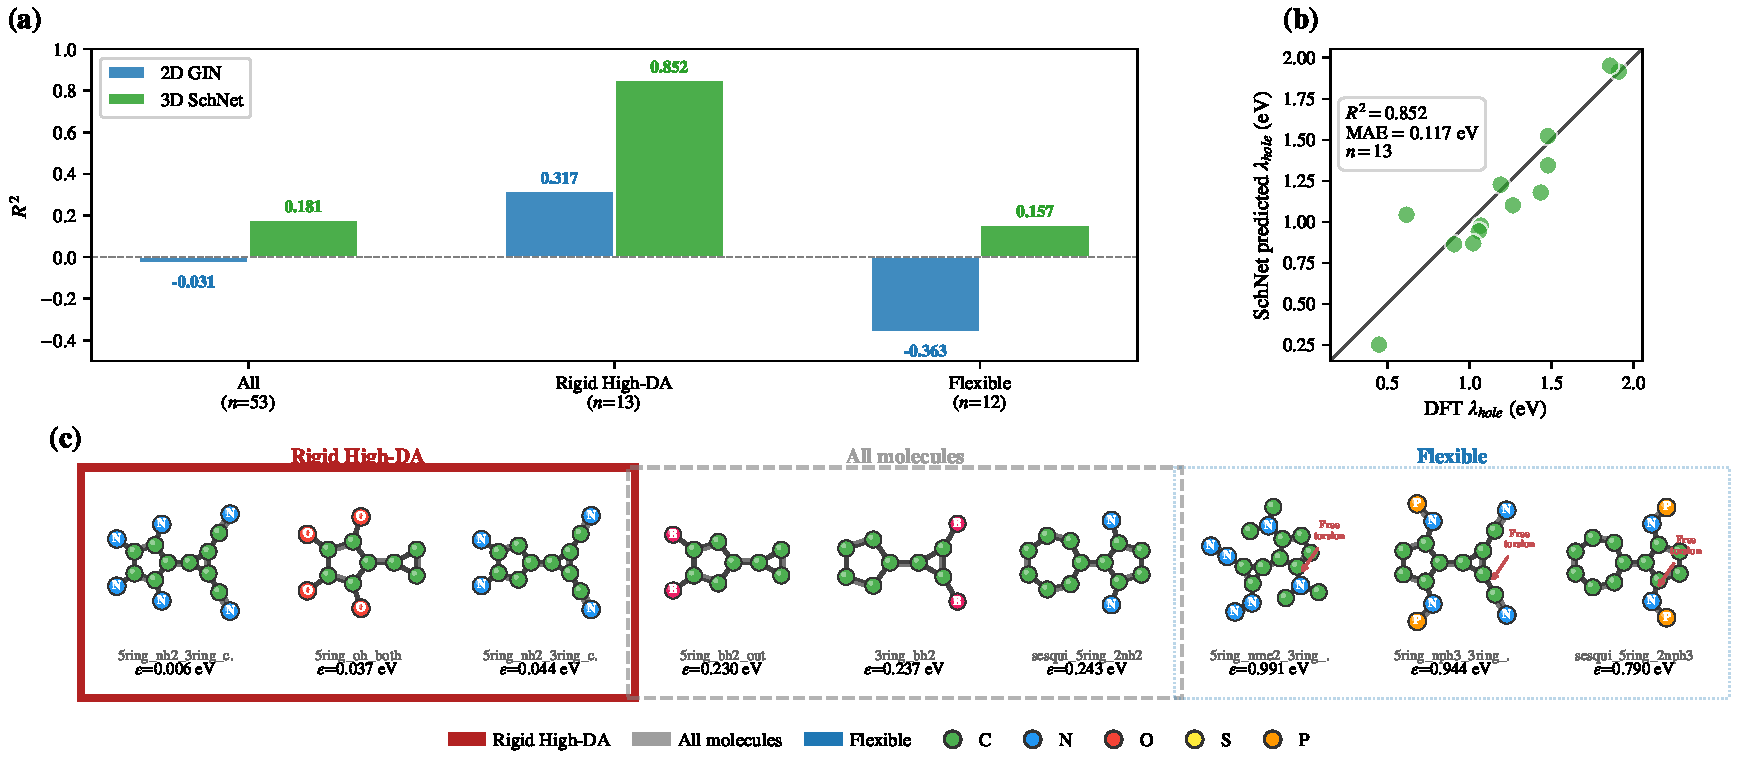
\includegraphics[width=\columnwidth]{../results/figures/fig17_subgroup_analysis.pdf}
\caption{Subgroup analysis of Client~D predictions.
(a)~$\Rsq$ comparison across subgroups for GIN and SchNet encoders.
(b)~Predicted vs.\ true $\lamhole$ scatter plot for the rigid high-DA subgroup ($n = 13$, SchNet $\Rsq = 0.852$).
(c)~Representative molecules from each subgroup with 2D ball-and-stick representations; green border = rigid high-DA, grey border = all molecules, red border = flexible.}
\label{fig:subgroup}
\end{figure}

% ================================================================
%  CONCLUSIONS
% ================================================================
\section{Conclusions}\label{sec:conclusions}

This work has presented FedPer-KAN, a personalized federated learning framework for predicting molecular reorganization energy ($\lam$) across four heterogeneous clients spanning non-aromatic small molecules, aromatic compounds, conjugated organic semiconductors, and TADF emitters.
Through 15 systematic experiments and four ablation studies, the following principal findings are established.

\textbf{(1) Personalized federated learning enables effective cross-domain $\lam$ prediction.}
The combination of \FedPer{}~\cite{Arivazhagan2019_FedPer} and \FedBN{}~\cite{Li2021_FedBN} strategies---sharing encoder parameters $\thetaenc$ while keeping regression heads $\thetahead$ and batch normalization statistics private---yields consistent improvements across all clients.
Client~B achieves $\Rsq = 0.854$ under the federated GIN+KAN framework (E8), compared to $\Rsq = 0.686$ for the local baseline (E2), representing a 24.5\% improvement.
Even the data-scarce Client~D benefits: its $\Rsq$ shifts from $-0.68$ (local, E5) to $+0.03$ (federated 3-client, E8), crossing from meaningless to weakly informative predictions.

\textbf{(2) KAN regression heads outperform MLPs as personalized physical mappers.}
Replacing MLP heads with Kolmogorov--Arnold Network (KAN) heads~\cite{KAN2024} improves Client~A $\Rsq$ from 0.523 (E1, MLP) to 0.683 (E4, KAN)---a 30.7\% relative gain---under otherwise identical local training conditions.
The KAN's learnable spline-based activation functions are better suited to capturing the non-linear mapping from graph embeddings to $\lam$, and their compact parameterization (188K parameters) makes them particularly appropriate as client-private modules in the federated setting.

\textbf{(3) 2D graph representations exhibit a fundamental information bottleneck for conformationally flexible molecules.}
Systematic hypothesis testing (Section~\ref{sec:bottleneck}) reveals that neither data scarcity, target-quantity mismatch, nor chemical-space divergence accounts for the poor Client~D predictions under 2D GIN encoding.
Rather, the inability of topological graphs to encode dihedral angles, steric interactions, and torsional barriers---the physical quantities governing $\lam$ in flexible donor--acceptor systems---constitutes the primary limitation.
Per-molecule analysis provides direct evidence: GIN errors correlate with the number of rotatable bonds ($r = 0.30$, $p = 0.028$), whereas 3D SchNet errors do not ($p = 0.256$).

\textbf{(4) 3D SchNet encoding partially breaks the bottleneck within the federated framework.}
Replacing the GIN encoder with SchNet~\cite{Schutt2018_SchNet} improves Client~D $\Rsq$ from $-0.031$ (E12) to $+0.181$ (E14), the largest single-factor improvement observed in our study ($\Delta \Rsq = +0.212$).
SchNet outperforms GIN on 67.9\% of Client~D molecules, with the advantage concentrated on conformationally flexible structures.
This result indicates that 3D information, even from approximate force-field conformers, provides a qualitative advance over 2D representations.

\textbf{(5) Subgroup analysis reveals that for rigid donor--acceptor molecules, federated SchNet achieves $\Rsq = 0.852$, confirming that the remaining error on the full set originates from force-field conformational uncertainty rather than architectural limitations.}
Stratifying Client~D by molecular rigidity and donor--acceptor character reveals that the rigid high-DA subgroup ($n = 13$, donor fraction $\geq 0.25$, $n_{\text{rot}} = 0$) achieves $\text{MAE} = 0.117$~eV, approaching centralized benchmarks~\cite{Li2023_SchNet}.
The $\Delta \Rsq = +0.535$ between SchNet and GIN on this subgroup---more than double the full-set gain---confirms that 3D encoding is maximally effective when force-field conformers faithfully represent the true geometry (Section~\ref{sec:subgroup}).

\paragraph{Limitations.}
Several limitations of the current study should be acknowledged.
The absolute predictive accuracy for Client~D ($\Rsq = 0.181$, $\text{MAE} = 0.304$~eV) falls short of practical chemical screening thresholds.
The RDKit MMFF94 force field provides only approximate conformers, particularly for the large donor--acceptor dihedral angles characteristic of TADF emitters; DFT-optimized geometries would likely improve 3D model performance.
In addition, the current framework does not incorporate formal privacy guarantees such as differential privacy or secure aggregation, which would be necessary for deployment with genuinely proprietary data.

\paragraph{Future directions.}
Several avenues for improvement are apparent.
Expanding the TADF dataset through additional DFT calculations would address the data scarcity issue.
Replacing SchNet with equivariant 3D GNNs such as DimeNet++~\cite{Gasteiger2020_DimeNet} or PaiNN~\cite{Schutt2021_PaiNN} could improve angular sensitivity.
Substituting force-field conformers with DFT-optimized geometries---potentially generated via federated pre-training of a neural force field---would improve 3D input fidelity.
Finally, integrating differential privacy mechanisms into the federated aggregation protocol would enable genuinely privacy-preserving collaborative learning across pharmaceutical and materials-science institutions.

% ================================================================
%  PLACEHOLDER SECTIONS
% ================================================================

% \section*{Declarations}
% \paragraph{Availability of data and materials}
% All code and data are available at \url{https://github.com/lengcan276/FedSchNet-ReorgEnergy}.

% \paragraph{Competing interests}
% The authors declare no competing interests.

% ================================================================
%  REFERENCES
% ================================================================
\bibliographystyle{unsrt}
\bibliography{references}

% ================================================================
%  FIGURE AND TABLE PLACEHOLDERS (for cross-referencing)
% ================================================================
% These will be positioned properly once all sections are written.

\clearpage
\appendix
\section*{Figures and Tables Referenced in the Text}

\begin{figure}[h]
\centering
% 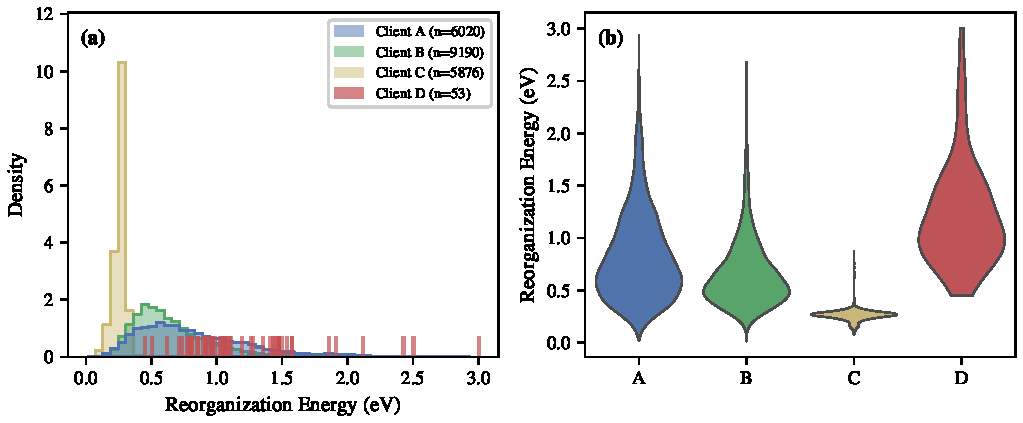
\includegraphics[width=\columnwidth]{../results/figures/fig2_dataset_distribution.pdf}
\caption{Dataset overview: molecular weight distributions and label ($\lam$) ranges for all four clients.
Client~D exhibits the broadest $\lamhole$ range (0.45--3.00~eV), reflecting the conformational diversity of TADF emitters.}
\label{fig:dataset}
\end{figure}

\begin{figure}[h]
\centering
% 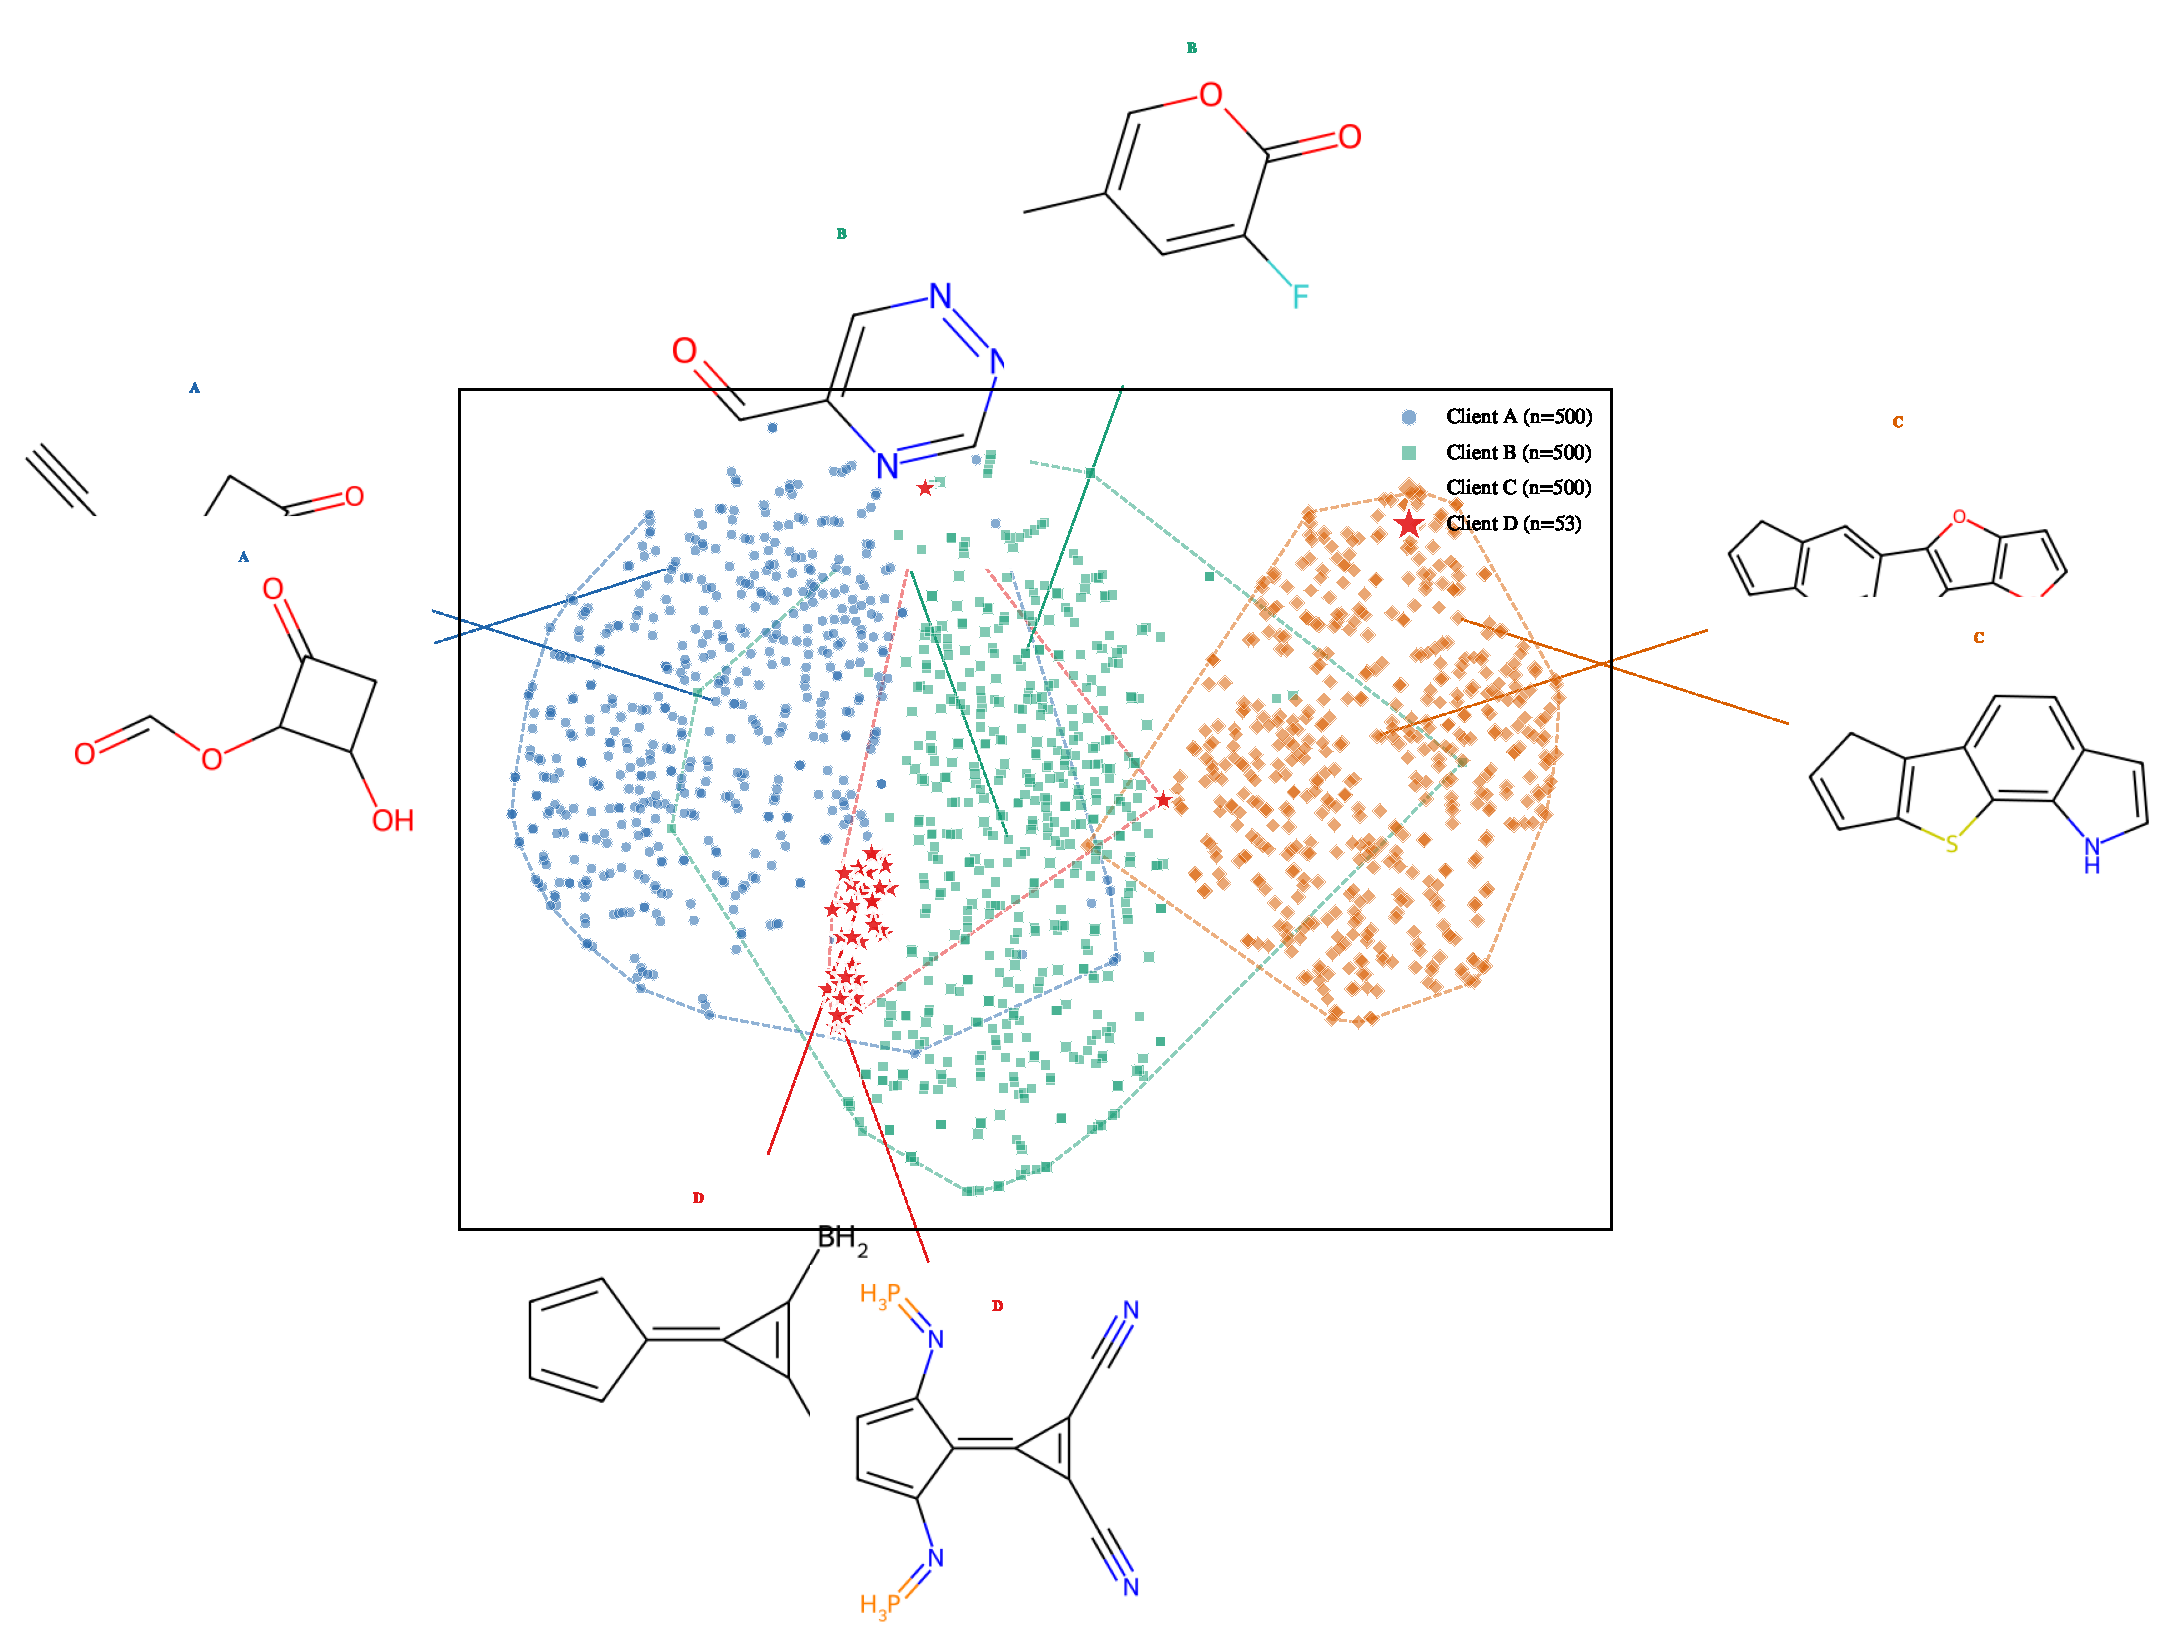
\includegraphics[width=\columnwidth]{../results/figures/fig4_tsne.pdf}
\caption{t-SNE visualization of Morgan fingerprint chemical space.
Client~D (TADF) occupies a distinct region characterized by complex donor--acceptor architectures.
Client~C (conjugated semiconductors) bridges the gap between the QM9-derived Clients~A/B and Client~D.}
\label{fig:tsne}
\end{figure}

\begin{figure}[h]
\centering
% 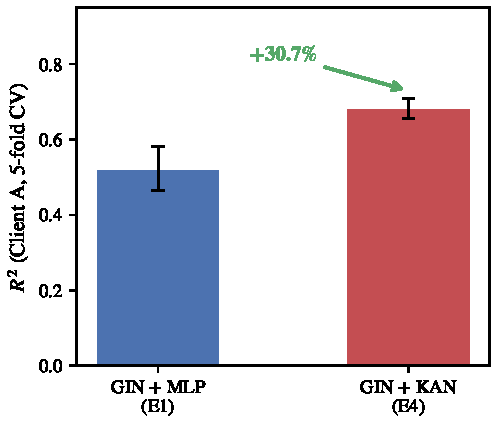
\includegraphics[width=\columnwidth]{../results/figures/fig5_kan_vs_mlp.pdf}
\caption{Comparison of KAN vs.\ MLP regression heads under local training conditions.
KAN outperforms MLP by 30.7\% in $\Rsq$ on Client~A (E4 vs.\ E1).}
\label{fig:kan_vs_mlp}
\end{figure}

\begin{figure}[h]
\centering
% 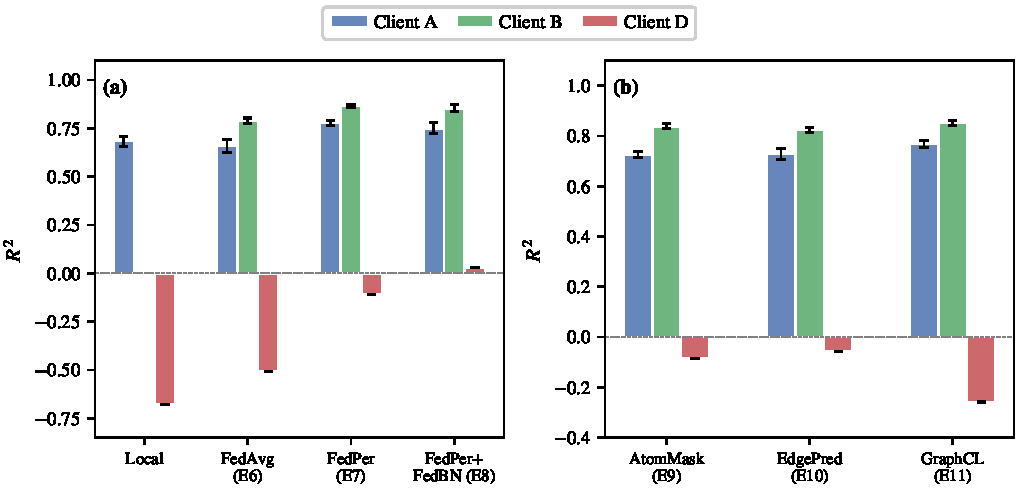
\includegraphics[width=\columnwidth]{../results/figures/fig6_strategies_ssl.pdf}
\caption{(a) Federated strategy comparison: Local, \FedAvg{}, \FedPer{}, \FedPer{}+\FedBN{} for GIN+KAN.
(b) Self-supervised pre-training methods: AtomMask, EdgePred, GraphCL.}
\label{fig:strategies}
\end{figure}

\begin{figure}[h]
\centering
% 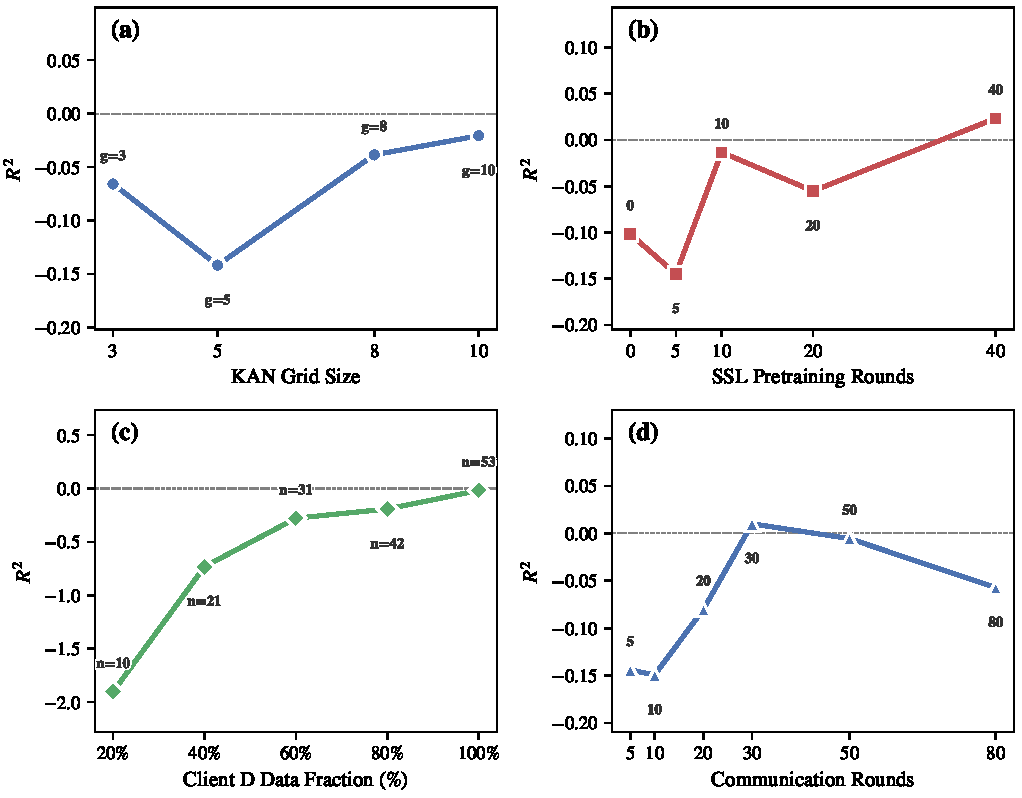
\includegraphics[width=\columnwidth]{../results/figures/fig9_ablation_combined.pdf}
\caption{Ablation studies on Client~D $\lamhole$ $\Rsq$:
(a) KAN grid size, (b) SSL pre-training rounds, (c) data size, (d) communication rounds.}
\label{fig:ablation}
\end{figure}

\begin{figure}[h]
\centering
% 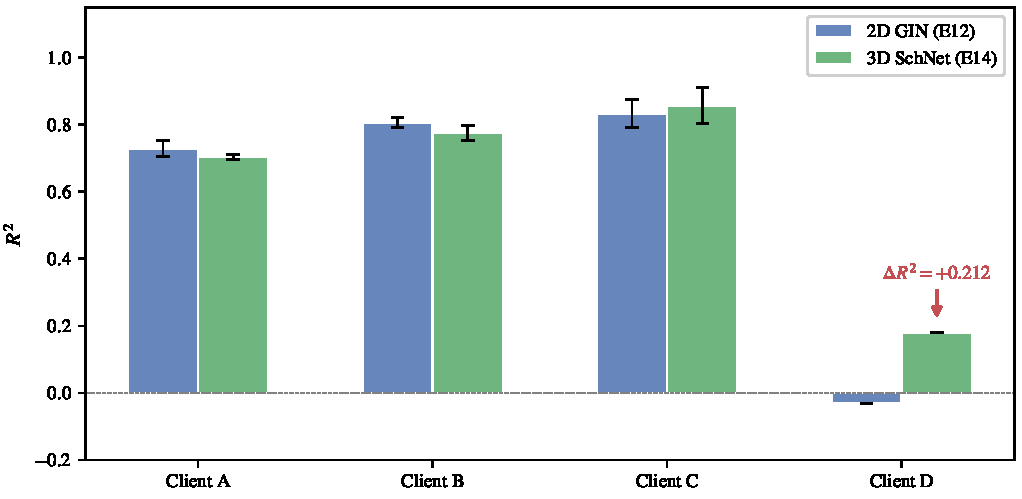
\includegraphics[width=\columnwidth]{../results/figures/fig13_gin_vs_schnet.pdf}
\caption{Comparison of 2D GIN (E12) vs.\ 3D SchNet (E14) across all clients.
SchNet provides the largest improvement on Client~D ($\Delta \Rsq = +0.212$).}
\label{fig:gin_vs_schnet}
\end{figure}

\begin{figure}[h]
\centering
% 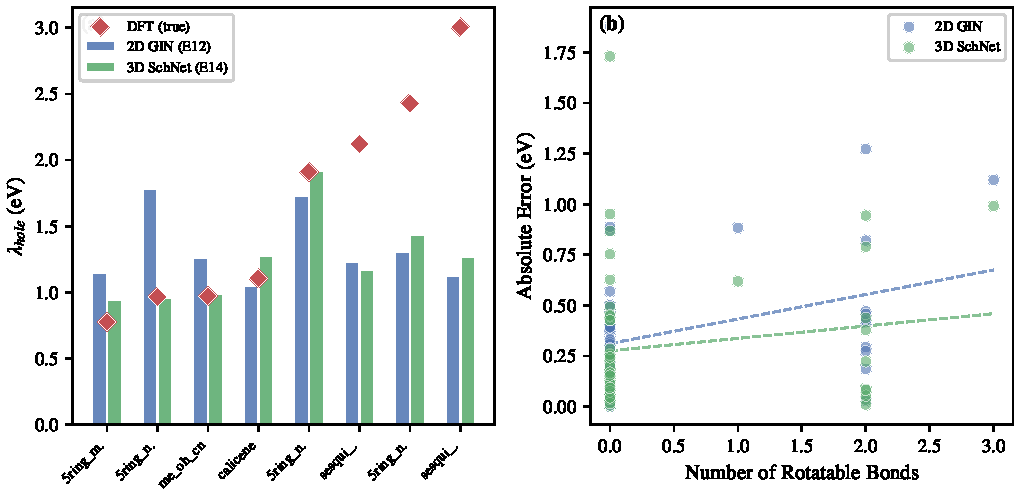
\includegraphics[width=\columnwidth]{../results/figures/fig15_case_study.pdf}
\caption{Per-molecule case study on Client~D.
(a) Predicted vs.\ true $\lamhole$ for eight representative molecules.
(b) Absolute error vs.\ number of rotatable bonds for all 53 molecules;
GIN errors show a significant positive correlation ($r = 0.30$, $p = 0.028$), SchNet errors do not ($p = 0.256$).}
\label{fig:case_study}
\end{figure}

\begin{figure}[h]
\centering
% 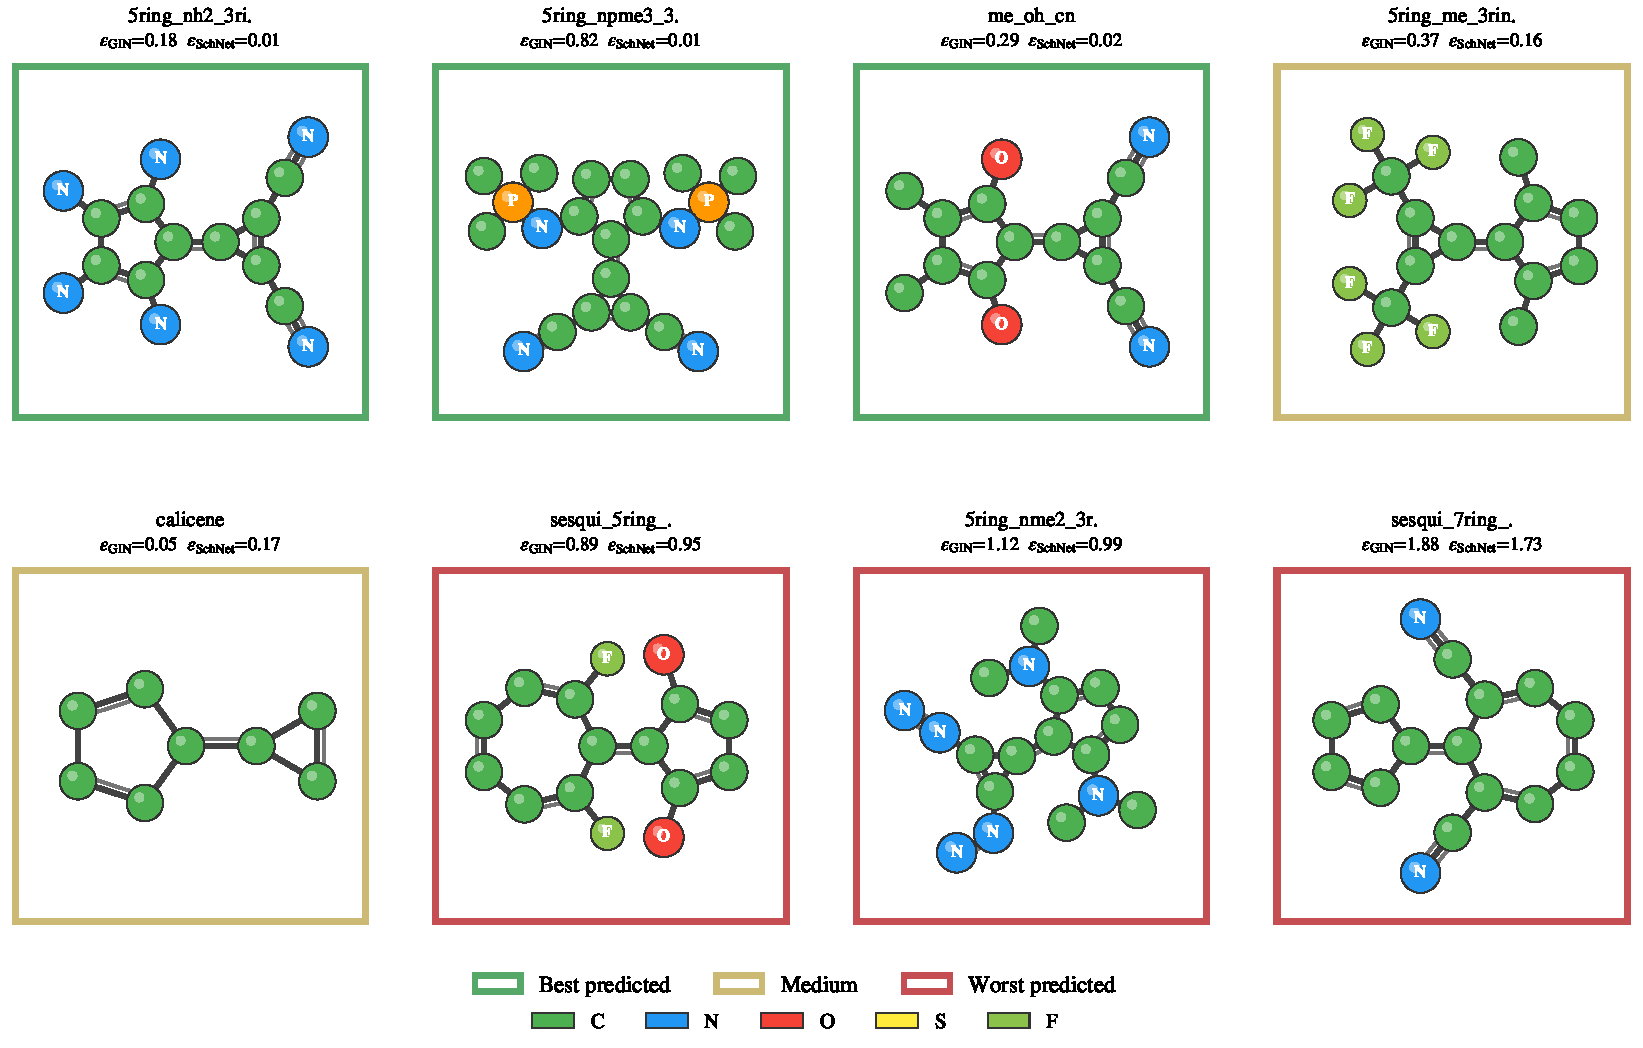
\includegraphics[width=\columnwidth]{../results/figures/fig16_representative_molecules.pdf}
\caption{Ball-and-stick representations of eight representative Client~D molecules,
categorized by SchNet prediction quality: best (green border), medium (gold), and worst (red).}
\label{fig:representative_mols}
\end{figure}

\begin{figure}[h]
\centering
% 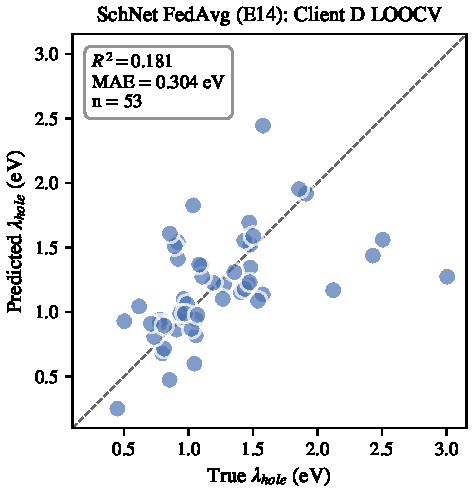
\includegraphics[width=\columnwidth]{../results/figures/fig14_scatter.pdf}
\caption{Scatter plot of predicted vs.\ true $\lamhole$ for the best-performing model (E14, SchNet+KAN \FedAvg{}) on Client~D.}
\label{fig:scatter}
\end{figure}

\begin{table}[h]
\centering
\caption{Summary of key experimental results. Values reported as mean$\pm$std over 5-fold CV (Clients~A, B, C) or single LOOCV run (Client~D). New experiment IDs (E1--E15) are used; see Supplementary Table~S1 for mapping to internal IDs.}
\label{tab:summary}
\small
\begin{tabular}{@{}llcccc@{}}
\toprule
ID & Configuration & $\Rsq_\text{A}$ & $\Rsq_\text{B}$ & $\Rsq_\text{C}$ & $\Rsq_\text{D,h}$ \\
\midrule
E1 & Local GIN+MLP A          & 0.523 & ---   & ---   & ---    \\
E4 & Local GIN+KAN A          & 0.683 & ---   & ---   & ---    \\
E5 & Local GIN+KAN D          & ---   & ---   & ---   & $-$0.677 \\
E6 & \FedAvg{} GIN+MLP        & 0.660 & 0.789 & ---   & $-$0.507 \\
E7 & \FedPer{} GIN+KAN        & 0.777 & 0.865 & ---   & $-$0.108 \\
E8 & \FedPer{}+\FedBN{} GIN+KAN & 0.750 & 0.854 & ---   & $+$0.028 \\
E12 & \FedPer{}+\FedBN{} 4-Cl. GIN+KAN & 0.729 & 0.807 & 0.833 & $-$0.031 \\
E13 & Centralized SchNet+KAN  & ---   & ---   & ---   & $-$0.004 \\
E14 & \FedAvg{} SchNet+KAN    & 0.704 & 0.775 & 0.857 & $+$0.181 \\
E15 & \FedPer{} SchNet+KAN    & 0.703 & 0.778 & 0.879 & $+$0.139 \\
\bottomrule
\end{tabular}
\end{table}

\end{document}
